\documentclass[a4paper]{article}

%% Language and font encodings
\usepackage[french]{babel}
\usepackage[utf8x]{inputenc}
\usepackage[T1]{fontenc}

%% Sets page size and margins
\usepackage[a4paper,top=3cm,bottom=3cm,left=2cm,right=2cm,marginparwidth=2cm]{geometry}

%% Useful packages
\usepackage{amsmath}
\usepackage{graphicx}
\usepackage[colorinlistoftodos]{todonotes}
\usepackage[colorlinks=true, allcolors=black]{hyperref}
\usepackage{fourier-orns}
\usepackage{titlesec}
\usepackage{fancyhdr}
\usepackage{fancyvrb}
\usepackage{float}
\pagestyle{fancy} 
\setcounter{tocdepth}{5}

%% Tikz stuff
\usepackage{tikz}
\usetikzlibrary{calc, arrows}
\tikzstyle{incolore} = [rectangle, rounded corners, draw=black, minimum height=1cm, minimum width=3cm, text width=3cm, text centered]

\usepackage{libertine}
\newcommand{\hsp}{\hspace{20pt}}
\newcommand{\HRule}{\rule{\linewidth}{0.5mm}}

\renewcommand{\headrulewidth}{1pt}
\fancyhead[C]{} 
\fancyhead[L]{}
\fancyhead[R]{\footnotesize{\leftmark}}

\renewcommand{\footrulewidth}{1pt}
\fancyfoot[C]{}
\fancyhead[L]{}
\fancyfoot[R]{\thepage}

\definecolor{Zgris}{rgb}{0.87,0.85,0.85}

\usepackage{eso-pic,graphicx}
\usepackage{xcolor}
\newcommand{\bgimg}[1]
{
    \AddToShipoutPicture
    {
        \put(\LenToUnit{0 cm},\LenToUnit{0 cm})
        {
            \includegraphics[width=\paperwidth,height=\paperheight]{#1}
        }
    }
}
\begin{document}





\begin{titlepage}
    \begin{sffamily}
        \begin{center}
            
\includegraphics[width=5cm]{images/LogoHenallux.PNG}~\\[1.5cm]
            \textsc{\Large Rapport de laboratoire}\\[1.5cm]

            % Title
            \HRule \\[0.4cm]
            { \huge \bfseries Huitième laboratoire : Analyse de signaux radio FM\\[0.4cm] }
            \HRule \\[2cm]

            % Author and supervisor
            \begin{minipage}{0.4\textwidth}
                \begin{flushleft} \large
                    Roumache Grégoire\\
                    Sénéchal Julien\\
                    Robert Alexandre\\
                    Wallemme Maxime\\
                    Kenmeugne Lionel\\
                    Didion Charles
                \end{flushleft}
            \end{minipage}
            \begin{minipage}{0.55\textwidth}
                \begin{flushright} \large
                    Laboratoire de sciences appliquées à l'informatique\\
                    Sécurité des systèmes, technologie de l'informatique\\
                    Hénallux\\
                    Première année, groupe H \\
                    Année académique 2019-2020\\
                \end{flushright}
            \end{minipage}
            \vfill

            % Bottom of the page
            {\large 30 Avril 2020}
        \end{center}
    \end{sffamily}
\end{titlepage}







\let\cleardoublepage\clearpage















\section{Introduction}





Dans ce rapport, nous allons parler un peu des fréquences radios. Comment se fait-il qu’une radio sois capable de monter le son lors des annonces trafic ? Et comment la sécurité des communications radio peut-elle être assurée ? RSD, WFM, FFT, des abréviations qui à première vue n’ont pas beaucoup de sens. Mais qui, pourtant, assure la base de toute les communications radio actuelle.















\section{Rappels théoriques}










\subsection{Qu’est-ce que RDS ?}





Qu’est-ce que le Radio Data System ? “RDS” = service de transmission de données numériques qui est également une norme européenne. Développé en 1974 par plusieurs entreprises de radiodiffusions et basé sur son prédécesseur l’ARI (Autofahrer-Rundfunk-Informationssystem).

Il est composé de plusieurs fonctionnalités toute lié à des sous programmes internes:
\begin{itemize}
    \item Programme service (PS)
    \item Alternative Frequencies (AF)
    \item Clock time (CT)
    \item Traffic programme (TP)
    \item Traffic annoncement (TA)    
\end{itemize}
 
\begin{enumerate}
    \item Le programme service (PS): fonctionnalité qui permet d’afficher le nom de la station radio active. À la base 8 caractères alphanumérique maximum par après détourner de la norme pour avoir accès au nom du titre de la musique jouer au moment de l’écoute.
    \item Alternative Frequencies (AF): partie logicielle qui se calibre automatiquement sur la meilleure fréquence possible d’écoute (évite les coupures radios quand le véhicule est en mouvement.
    \item Le Clock Time (CT): service qui calibre l’heure de l’appareil de manière automatique prenant en compte les changements d’heures.
    \item Trafic Programme (TP): l’icône qui indique s'il y a des annonces concernant le trafic routier sur cette station.
    \item Traffic annoncement (TA): annonce quand une information sur le trafic a lieu et augmente le volume pour qu’elle soit facilement audible.
\end{enumerate}










\subsection{Que veux dire WFM ?}





\paragraph{}
Il existe 3 types de bandes FM :
\begin{itemize}
    \item \emph{FM} : Frequency Modulation
    \item \emph{WFM} : Wide Frequency Modulation
    \item  \emph{NFM} : Narrowband Frequency Modulation
\end{itemize}

\emph{\textbf{WFM}} signifie \emph{Wide FM}, autrement dit \emph{FM à bande large}. C'est ce qui est utilisé pour la diffusion de
la radio en \emph{FM} (88 - 108 Mhz). Le \emph{FM}, lui, est une modulation a bande étroite.
Etant donné que le \emph{WFM} a une bande plus large, il y a moyen de faire du Stereo.

\begin{figure}[H]
    \centering
    \includegraphics[width = 7cm]{images/imagesfm.jpg}
    \caption{Différence de bande passante entre \emph{FM}, \emph{WFM}, et \emph{NFM}}
\end{figure}










\subsection{Que représente le paramètre FFT ?}





FFT est l'acronyme de \textit{Fast Fourier Transform}. La transformation de Fourier rapide est un algorithme qui sert à calculer la transformation de Fourier discrète. L'utilisation de cet algorithme est beaucoup plus rapide que l'utitilisation d'un algorithme naïf:
\begin{itemize}
    \item complexité du FFT: $ O(n \log n) $;
    \item complexité de l'algorithme naïf: $ O(n^2) $.
\end{itemize}
Modifier le paramètre \textit{FFT size} (taille de la transformation rapide de Fourier) peut aider à mieux visualiser la fréquence ou le domaine temporel.










\subsection{Quel moyen mettriez-vous en œuvre pour vous protéger contre une usurpation de bande de fréquence ?}





L’usurpation de bande de fréquence est un type d’attaque parmi d’autres sur les fréquences radio. Le terme généralement utilisé pour l’usurpation est le "spoofing". Deux autres types d’attaques comme le "brouillage" ou "l’écoute passive" peuvent être utilisés. Le brouillage consiste à émettre un bruit sur la fréquence radio à l’aide d’un amplificateur.

L’écoute passive quant à elle, consiste pour l’attaquant à prendre connaissances de données transmises entre l’émetteur et le récepteur de la fréquence radio. Concernant le spoofing (usurpation de bande de fréquences), cela va consister à modifier les valeurs, ou données transmises afin d’atteindre la disponibilité du système. Pour contrer cette attaque, on peut protéger la bande de fréquence radio à l’aide d’une authentification par challenge-réponse.

Cette méthode est bien connue dans le milieu de la sécurité informatique, elle consiste à ce qu’une partie pose un challenge et l’autre partie doit y répondre à l’aide d’un algorithme ou autres et de manière correcte afin de valider l’authentification.


\textbf{Exemple}: Algorithme utilisé: $ a \times b - 1 $ \\
Challenge :
\begin{center} \begin{tabular}{c|c|c|c|c}
    1 & 5 & 6 & 9 & 7 \\
    a & b & c & d & e
\end{tabular} \end{center}
Réponse : \begin{center} $ 1 \times 5 - 1 = 4 $ \end{center}

Le système ou la personne qui envoie le challenge change évidemment à chaque demande d’authentification, les chiffres envoyés. Ainsi, l’attaquant ne possédant pas l’algorithme, il ne pourra pas pénétrer dans le système.

\begin{figure}[H]
    \centering
    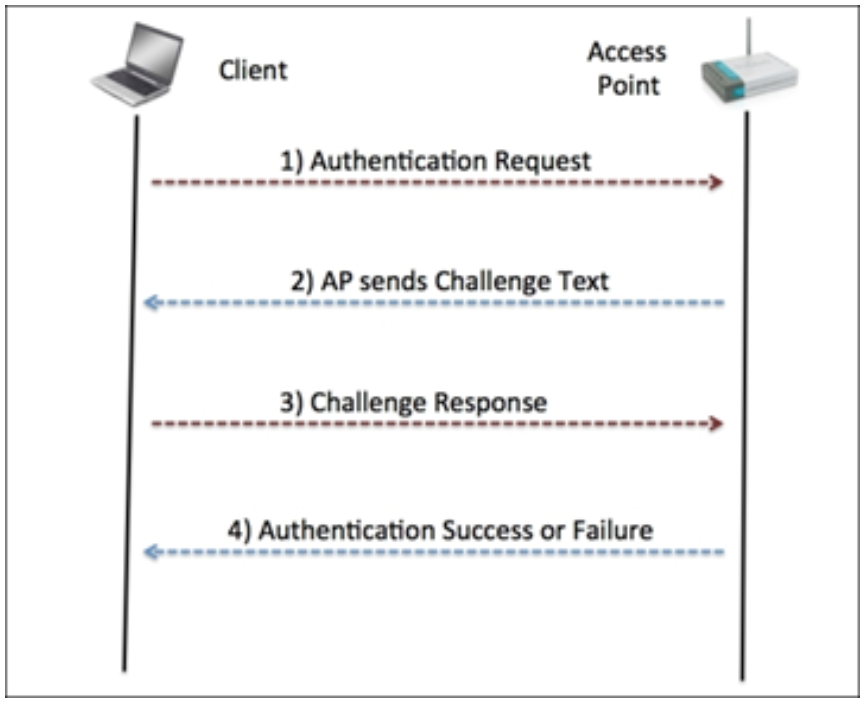
\includegraphics[width=0.4\textwidth]{images/Capture001.PNG}
    \caption{Schéma du dialogue entre le client et le point d'accès}
    \label{}
\end{figure}













\section{Conclusion}





Le \textbf{Radio Data System} (RDS) est un service de transmission de données numériques en parallèle des signaux audio et \textbf{la gestion de la main-d'œuvre} (WFM) est un processus institutionnel qui maximise les niveaux de performance et les compétences d'une organisation. La \textbf{transformation de Fourier rapide} (\textbf{FFT}) quant à lui est un algorithme de calcul de la transformation de Fourier discrète (TFD). Toutes ces notions nous ont amenées à nous poser des questions sur les risques ou attaques affectant les fréquences radio. D’où l’usurpation de bande de fréquence (spoofing), le brouillage ou l’écoute passive que nous avons développés mais qui sont des types d’attaques parmi d’autres.














\newpage \tableofcontents \listoffigures
\begin{thebibliography}{9}
\bibitem{1} https://www.forumatena.org/files/livresblancs/L\%27environnement\%20sans\%20fil.pdf
\bibitem{2} https://www.youtube.com/watch?v=19CE1yeKzjU
\bibitem{3} https://searchsecurity.techtarget.com/definition/challenge-response-system
\bibitem{4} https://www.ornikar.com/code/cours/mecanique-vehicule/technologie-assistance/radio-data-system
\bibitem{5} https://www.elttam.com/blog/intro-sdr-and-rf-analysis/
\bibitem{6} https://fr.wikipedia.org/wiki/Transformation\_de\_Fourier\_rapide
\bibitem{7} https://radiofreeq.wordpress.com/2016/06/21/fm-versus-nfm-for-best-radio-communications/
% \bibitem{8} 
\end{thebibliography}




















\end{document}
